%%%%%%%%%%%%%%%%%%%%%%%%%%%%%%%%%%%%%%%%%%%%%%%%%%%%%%%%%%%%%%%%%%%%%%
% How to use writeLaTeX: 
%
% You edit the source code here on the left, and the preview on the
% right shows you the result within a few seconds.
%
% Bookmark this page and share the URL with your co-authors. They can
% edit at the same time!
%
% You can upload figures, bibliographies, custom classes and
% styles using the files menu.
%
%%%%%%%%%%%%%%%%%%%%%%%%%%%%%%%%%%%%%%%%%%%%%%%%%%%%%%%%%%%%%%%%%%%%%%

\documentclass[12pt]{article}

\usepackage{sbc-template}

\usepackage{graphicx,url}

\usepackage{algorithm,algorithmic}
\usepackage{listings}

\makeatletter
\renewcommand{\ALG@name}{Algoritmo}
\renewcommand{\refname}{Refer\^encias}
\makeatother


\usepackage{algpseudocode}


%\usepackage[brazil]{babel}   
\usepackage[utf8]{inputenc}  
     
\sloppy

\title{Uma análise comparativa entre algorítimos estáticos para balanceamento de carga em redes SDN em ambiente IoT}

\author{Anselmo L. E. Battisti\inst{1}, Gabriel Carrara\inst{1}}

\address{Instituto de Computação -- Universidade Federal Fluminense (UFF)}

\begin{document} 

\maketitle

\begin{resumo} 
As redes de comunicação de dados são fundamentais para a implantação das Cidades Inteligentes. Além delas fornecerem conectividade aos cidadãos, é a partir da infraestrutura de redes que os inúmeros sensores enviam dados para as centrais de processamento. Um dos requisitos fundamentais para a implantação de uma infraestrutura de IoT é a escalabilidade da rede de trasmissão de dados. Uma das alternativas para melhorar a escalabilidade de uma rede é a implantação de mecanismos de balanceamento de carga. Nesse trabalho foram analisadas três técnicas diferentes para balanceamento estático do tráfego em uma rede SDN. Foi observado que o balanceamento utilizando Round Robin com peso foi x\% mais eficiente em comparação com os seus rivais no que diz respeito ao tempo de resposta.
\end{resumo}

\begin{abstract}
    
\end{abstract}

\section{Introdução}


\section{Referencial Teórico}

Nessa sessão será apresentada uma visão geral sobre os principais conceitos e tecnologias abordados nesse trabalho. Os principais temas abordados são: Cidades Inteligentes; Internet da Coisas. Redes definidas por software e balanceamento de carga. Também apresentaremos nessa sessão algumas tecnologias já propostas com o objetivos similares ou complementares ao IoTBalance. 

\subsection{Cidades Inteligentes}

O crescente aumento da população urbana demandou ao longo da história que tecnologias fossem desenvolvidas para pudesse existir o bem estar social. Em seu artigo \cite{Caragliu2011} apresenta uma agenda com alguns tópicos estratégicos que devem ser analisados para uma cidades possa ser chamada de inteligente. No Brasil a realidade do aumento da população urbana também é constatada de acordo com o \cite{IBGE2011}.

Além dos aspectos sociais apontados por \cite{Caragliu2011}, também podemos analisar as Cidades Inteligentes sobre aspectos mais técnicos da sua implementação. \cite{Gharaibeh2017} apresenta em seu trabalho uma visão geral sobre as principais tecnologias que permitiriam a criação deste tipo de ambiente. Dentre elas, podemos destacar: Internet das coisas; gestão e segurança dos dados; virtualização de funções de rede; computação nas nuvens e redes definidas por software. 

O simples uso da da tecnologia não garante que uma cidade seja inteligente. Em seu trabalho \cite{Anttiroiko2014} propõe uma classificação para cidades inteligentes onde existe uma correlação direta entre o emprego adequado das tecnologias da informação com a qualidade de vida dos sujeitos. Como tônica de sua pesquisa ele apresenta que a comunicação entre os sistemas é primeiro degrau que se deve alcançar para que uma cidade possa ser inteligente.

Nesse trabalho estamos buscando mecanismos que permitam que as redes de comunicação de uma cidade inteligente sejam escaláveis. Essa escalabilidade pode ser alcançada de diversas formas, aqui, estamos interessados no balanceamento de carga.

\subsection{Internet das Coisas}

Com o aumento da disponibilidade de mecanismos de transmissão de dados, tais como: WIFI, bluetooth, RFID, Li-Fi, 5G. É possível iniciar a coleta de dados de locais e ambientes onde antes não era possível. \cite{Ashton2009}  em 1999 em uma palestra na P&G foi um dos primeiros a utilizar o termo Internet das Coisas (IoT). Ele  acredita que a internet das coisas representa uma maneira de automatizar a coleta de informações do mundo real, uma vez que o ser humano tem limitação de tempo atenção e precisão quanto a coleta desse tipo de dados.

IoT pode mudar o mundo mais drasticamente do que a mudança ocorrida pelo desenvolvimento e posterior popularização da Internet tradicional.  


\subsection{Redes Definidas por Software (SDN)}

As redes de computadores passaram por diversas formas de organização ao longo das útlimas décadas. Recentemente, uma estratégia que vem sendo debatida pela comunidades acadêmica e implantada pela indústria são as SDN. Elas são uma nova abordagem para o gerenciamento de redes de computadores. Nelas, o hardware de encaminhamento de pacotes (\textit{switch}) conta com o apoio de um elemento centralizador chamado \textit{controller} que analisa os pacotes e decide sobre de que maneira os pacotes devem ser encaminhados. Essa abordagem segundo  \cite{Sezer_et_al_2013} apresenta alguns pontos importantes que devem ser analisados. Alguns deles são:

 \begin{itemize}
   \item Performance x flexibilidade:  CPU são mais flexíveis porém mais lentos do que circuítos de propósito específico usados nos encaminhadores de pacotes;
   \item Escalabilidade: existe um controlador central acessado por todos os encaminhadores de pacotes; 
   \item Segurança: como garantir em um ambiente com múltiplos usuários que a criação de novos fluxos não alterem os fluxos de outros usuários? Como tratar ataques de DDoS em um ambiente de propósito geral onde o controlador precisa analisar todos os pacotes que chegam até ele?
   \item Interoperabilidade: será necessária a introdução de novos protocolos que permitam a operação em paralelo de redes tradicionais e SDN em ambiente híbridos.
 \end{itemize}

%\textit{Software Defined Network} (SDN), seus fundamentos e principais desafios de implantação. SDN é um tipo de rede abstrata que permite uma otimização dos recursos da infraestrutura de redes tanto no que diz respeito à eficiência do uso dos diversos dispositivos e meios de transmissão de rede disponíveis, como dos recursos humanos. Segundo os autores, essas duas situações são otimizadas usando SDN pois é possível balancear a carga da rede, utilizando assim melhor os recursos disponíveis, além disso, esse balanceamento pode ser feito via software o que permite a um operador gerenciar um número maior de redes independentemente do local onde elas se encontram. SDN torna o processo de gerenciamento da infra de rede um processo muito mais relacionado com a configuração de software do que de configuração de hardware físicos, como originalmente era feito.

Entre as principais vantágens do uso de SDN temos: ....................

Um ponto crítico do uso de SDN é a existência de um ponto de falha central. Caso o \textit{controller} não esteja operacional, toda a rede ficará indisponível. Com o objetivo de aumentar a disponibilidade de uma rede SDN, \cite{Dixit2013} propõe uma estrutura onde existam múltiplos \textit{controllers} em uma rede SDN.

O uso de SDN em ambientes IoT vem sendo estudada. Em seu artigo \cite{7366932} apresenta uma abordagem chamada \textit{Black SDN}. O objetivo dessa tecnologia é aumentar a segurança em redes cujos dispositivos na maior parte do tempo esteja, hibernando e, apenas utilizem a rede em algum momento em particular. Os autores advogam que a tecnologia SDN permite a resolução de dois grandes problemas, o primeiro diz respeito a privacidade dos dados e o segundo diz respeito a localização dos recursos da rede. Os autores argumentam que uma das formas de mitigar a incidência de ataques sobre a privacidade dos dados é utilizar protocolos de segurança que criptografem os dados e metadados, além disso é necessário também criptografar os dados da camada de redes. Já para o problema de localização dos dispositivos eles sugerem que exista um controlador central que coordene o processo de troca de trafego entre os dispositivos. Com essa abordagem existe um mascaramento da origem e do destino do pacote, tornando assim anônima o processo de troca de dados entre dispositivos.

O artigo \cite{6819050} propôs uma nova arquitetura distribuída baseada no OpenFlow. Essa arquitetura tenta garantir a QoS fim-a-fim que é muito desejada em aplicações multimídia. A base da arquitetura proposta está na coleta e organização da topologia da rede e também do seu estado, tanto intra como inter domínios (AS), de tal forma que seja possível classificar o fluxo de dados de acordo com o nível de QoS necessário para que o usuário final fique satisfeito. Em uma cidade inteligente garantir qualidade de serviço é uma das tarefas centrais do administradores da rede.

O artigo \cite{Li2016} apresenta uma proposta de arquitetura horizontal para IoT utilizando SDN como meio de controle dos fluxos de dados. Segundos os autores, existe falta de interoperabilidade entre os diversos fabricantes de hardware e software para IoT, isso gera uma verticalização da infra-estrutura, ou seja, um tipo de sensor funciona para um certo tipo de domínio ou aplicação mas não para outro. Esse cenário, entre outras coisas gera dificuldade em inovação.  A proposta apresentada fornece mecanismos que permitem a interoperabilidade de dados, dispositivos e softwares pelo uso dos controladores SDN.

O uso de uma estrutura de redes desenvolvida com SDN permite, entre outras coisas, escalabilidade e a capacidade de inovação necessária dentro do contexto de redes que é necessário em uma cidade inteligente. Na próxima sessão falaremos sobre de que maneira o balanceamento de carga afeta a escalabilidade de uma rede.

\subsection{Balanceamento de Carga}

O balanceamento de carga em redes de computadores vem sendo estudado há algumas décadas. Em seu trabalho seminal \cite{Stentz1988} apresenta a formulação do problema e também um algorítimo para calcular o quão balanceada uma rede está.

O processo de balanceamento consiste em dividir de forma equitativa o tráfego de uma rede de acordo com algum critério estabelecido pelos gestores da rede. Algumas métricas que podem ser utilizadas para a definição do problema de balanceamento da rede são: tempo de resposta; vazão; perda de pacotes; custo; segurança da informação; etc.

Balanceamento de carga em redes de computadores segundo \cite{Peter2012} consiste em dividir o tráfego da rede entre diversos servidores sem que o usuário final perceba que essa divisão está acontecendo, como pode ser visto na  

A abordagem apresentada por \cite{Peter2012} utiliza um \textit{load balancer} no modo tradicional, como pode ser visto na Figura \ref{fig:balanceamento_carga_tradicional}. Nessa abordagem, existe um servidor a frente do switch interno da rede que faz o papel de ponte entre cada um dos servidores de conteúdo e o cliente. onde uma máquina física . Nesse trabalho estamos interessados em avaliar e analisar o balanceamento da carga da rede a partir da perspectiva do controlador de uma rede SDN. O controladores naturalmente já recebe solicitação de roteamento dos diversos switches da rede, sendo assim podemos usar as demandas do tipo \textit{packet-in} para disparar algoritmos para o adequado balanceamento da rede.

\begin{figure}[ht]
\centering
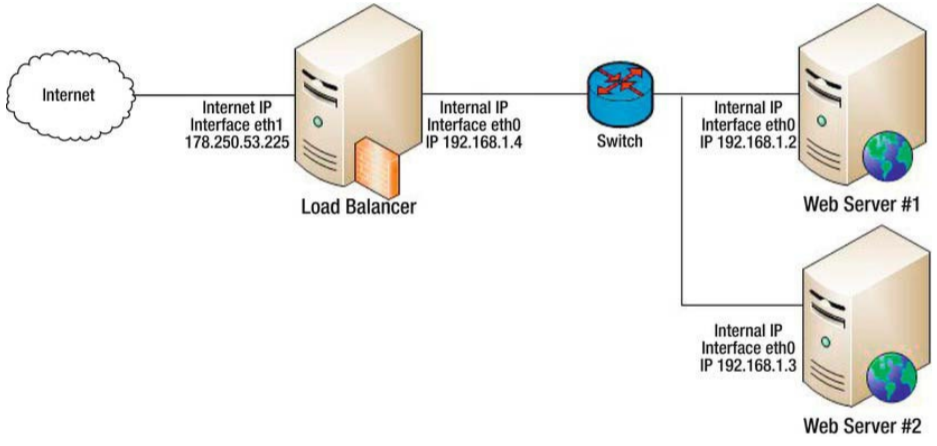
\includegraphics[width=0.8\textwidth]{images/load_balance.png}
\caption{Balanceamento de carga no modelo tradicional \cite{Peter2012}}
\label{fig:balanceamento_carga_tradicional}
\end{figure}

Podemos dividir os algorítimos de balanceamento de carga em dois grupos, os estáticos e os dinâmicos. Os algorítimos estático levam em consideração apenas os dados definidos no momento da sua concepção, parametrização e inicialização, ou seja, depois do início da sua operação o seu comportamento é baseado naquilo que ele sabia anteriormente, o Round Robin é um exemplo deste tipo de algorítimo. Já os algorítimos dinâmicos tomam a decisão sobre para quem enviar um processo de acordo com o estado atual da rede, nesse caso o balanceador de carga precisa obter informações sobre os servidores e links a fim de definir o destino de uma solicitação.

Nesse trabalho serão testadas três diferentes técnicas para o balanceamento de carga. 
\section{Apresentação do Método}

Nessa sessão serão serão apresentados os procedimentos metodológicos utilizados na elaboração e condução do experimento. 

\section{Técnicas de Balanceamento de carga analisadas}

Nesse trabalho foram testadas três técnicas distintas de balanceamento estático de carga em uma rede SDN, sendo eles:

\begin{itemize}
    \item Aleatório: nesse algorítimo o controlador SDN escolhe de forma aleatoria qual será o servidor responsável pelo processamento de uma solicitação;
    \item Round-Robin: nesse algorítimo o controlador SDN escolhe de forma sequencial qual será o próximo servidor que irá atender uma solicitação. A implementação utilizou uma lista circula para alcançar esse comportamento;
    \item Round-Robin com prioridade: nesse algorítimo o controlador SDN escolhe de forma sequencial qual será o próximo servidor que irá atender uma solicitação. A implementação utilizou uma lista circula para alcançar esse comportamento, porém, nesse cenário cada servidor tem pesos diferentes, ou seja, servidores com peso maior receberão mais requisições ao passo que servidores com peso menor receberão menos requisições,
\end{itemize}


\subsection{Estrutura da rede utilizada}

A rede 

\subsection{Hardware de Teste}

A fim de tornar os resultados dos testes o mais fidedignos possíveis optou-se por implantar o ambiente de teste em uma máquina virtual dedicada exclusivamente para a execução dos testes. A máquina foi hospedada em um datacenter da Digital Ocean. As configurações da mesma são as seguintes: 1GB de memória RAM; Processador Intel(R) Xeon(R) CPU E5-2650 v4 @ 2.20GHz.

O servidor roda o sistema operacional Ubuntu 18.04.1 LTS. 

\subsection{Software utilizados}

A rede foi simulada utilizando o a plataforma mininet na versão 2.3.0d4. O controlador escolhido para a execução dos testes foi o POX em sua versão 0.5.0 (eal). A escolha do tanto do mininet como do controlar POX deram-se em virtude da sua facilidade de aprendizado permitindo assim uma rápida prototipação dos testes.

A implementação dos algorítimos de balanceamento de carga foi feito utilizando como referência o \textit{script} pré-instalado do POX chamado "ip\_loadbalancer\.py" desenvolvido por James McCauley. Em sua versão original o \textit{script} implementa o balanceamento de carga utilizando o sorteio aleatório do servidor que será responsável pelo tratamento da requisição do usuário. Foi implementado o algorítimo Round Robin e o Round Robin com peso a fim de realizar as comparações.

\section{Resultados}


\section{Considerações Finais}

%Assistir Hai To Gensou No Grimgar - Episódio 02 Online
Nesse trabalho foi apresentada a estratégia do balanceamento de carga em uma rede SDN. O balanceamento de carga em uma rede minimiza diversos problemas, tais como: uso excessivo de uma única máquina, latência e disponibilidade de um serviço. Foram testadas três estratégias de balanceamento estático, sendo elas: aleatório. Round Robin e Round Robin com peso. Os resultados obtidos mostram que o o uso do ......

Para garantir a reprodutibilidade dos testes, os scripts utilizados para a execução do experimento podem ser acessados no github através do link: 

. We implemented load balancer using round robin strategy and compared it with already implemented random load balancer strategy. Results show that round robin strategy is better than random strategy. The other positive point about round-robin is that it is actually distributing the load uniformly while random is not. Limitation of our work is that we have not testing code on real hardware which might generate different results. Other Limitation is that code was tested using POX Controller. We did not use other controllers. SDN application’s performance is also dependent upon the performance of controller. This could be area for future research. One Major drawback in both round robin & random is that they do not take into consideration the current load on servers. Future works can involve load balancing based on server load using flow statistics

\bibliographystyle{sbc}
\bibliography{sbc-template}

\end{document}
